% ====================================================================
%+
% SECTION:
%    SolarSystem_AsteroidLightCurves.tex
%
% CHAPTER:
%    solarsystem.tex
%
% ELEVATOR PITCH:
%-
% ====================================================================

\section{Measuring Asteroid Colors}
\def\secname{\chpname:colors}\label{sec:\secname}

\credit{rhiannonlynne},
\credit{davidtrilling}

The varying compositions of asteroids result in a range of optical
colors. Sloan filters in general are sufficiently diagnostic to
discriminate among different compositional class
\citep[e.g.,][]{2008Icar..198..138P}.
Therefore, when a Solar System minor body is observed in $griz$ (Solar
System objects are generally quite faint in $u$ band and many fewer will
be detected),
% ; Y band xxx),
the color can be used to determine the
composition and, downstream, composition as a function of asteroid size,
family membership, orbital elements, or many other parameters.

% more motivation for color measurements?

One obstacle to determining asteroid colors is that asteroid rotation
periods are on the order of 2--20~hours, so that after an initial
measurement all further measurements (in the same filter, or other
filters) are obtained at an arbitrary rotational phase. Unless the
lightcurve is also known (perhaps determined from a large series of
measurements in the same bandpass, such as described in the section
above), multi-band measurements must occur at closely spaced times in
order to minimize the effects of the lightcurve on the measured color.

% --------------------------------------------------------------------

\subsection{Target measurements and discoveries}
\label{sec:\secname:targets}

% xx ref DelSanti, Peixinho 2015?16? xx
Analysis of existing databases of TNO multi-band measurements indicate
that pairs of high SNR measurements (SNR$>10$), acquired within a short
time period ($<2$ hrs) can provide a color measurement accurate to
within a few tenths
% (?)
of a magnitude.
% Currently only about xx (500?)
% xx TNOs have color measurements to this level of accuracy.


% --------------------------------------------------------------------

\subsection{Metrics}
\label{sec:\secname:metrics}

The metric {\tt ColorDeterminationMetric} searches for pairs of
observations, taken within a given number of hours, where the pair
contains observations in each of two specified filters above a
specified SNR (e.g., $g$ and $r$ band observations taken within 2
hours of each other, with SNR$>10$). If an object receives a minimum
number of pairs of observations (currently set to just a single pair
of observations), then it is considered as having that color
``measured.'' Thus, this metric can measure the fraction of the sample
population which receives an adequate color measurement, for a series
of colors.


% --------------------------------------------------------------------

\subsection{OpSim Analysis}
\label{sec:\secname:analysis}

\begin{figure}
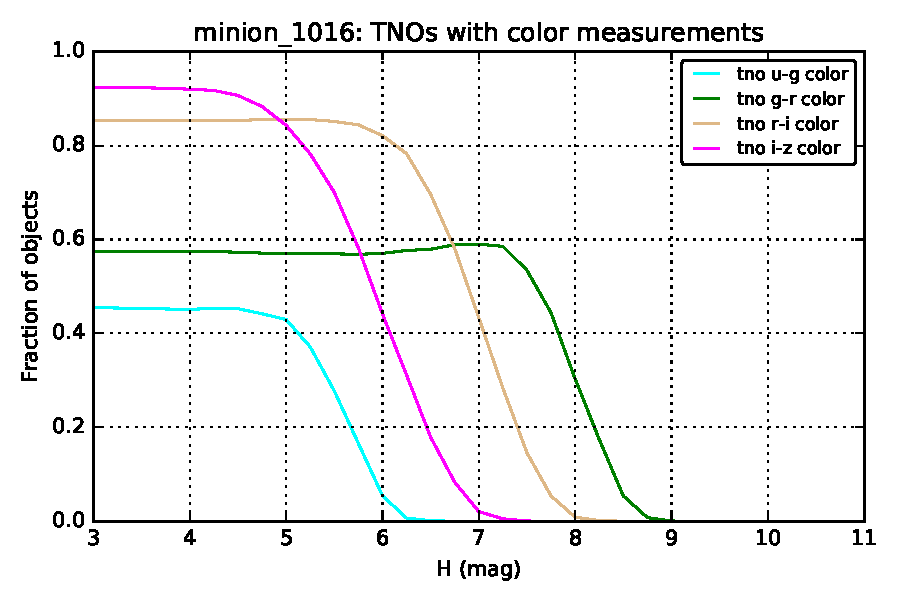
\includegraphics[width=3.3in]{figs/solarsystem/minion_1016_ColorDetermination_i-z_u-g_r-i_g-r_color_tno_MOOB_ComboMetricVsH}
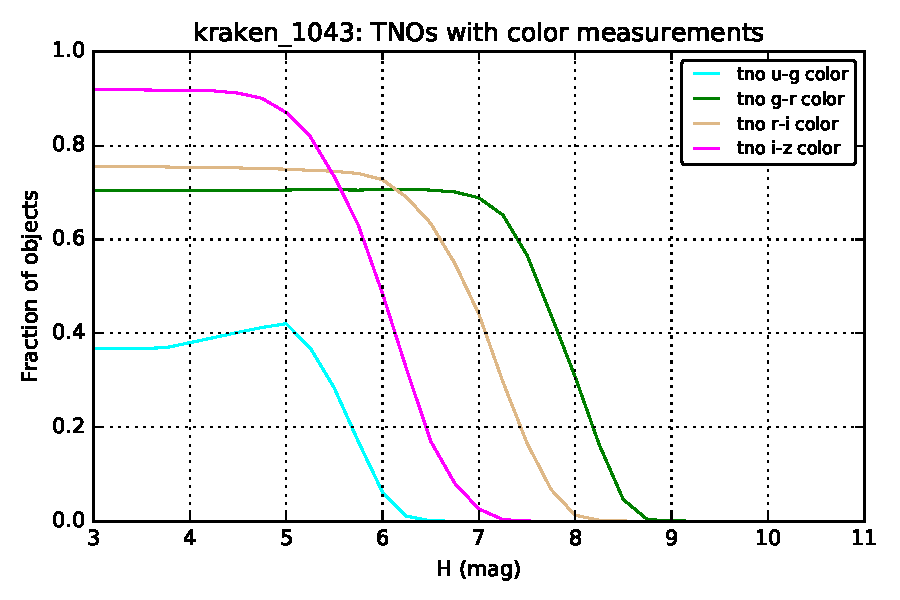
\includegraphics[width=3.3in]{figs/solarsystem/kraken_1043_ColorDetermination_i-z_u-g_r-i_g-r_color_tno_MOOB_ComboMetricVsH}
\\
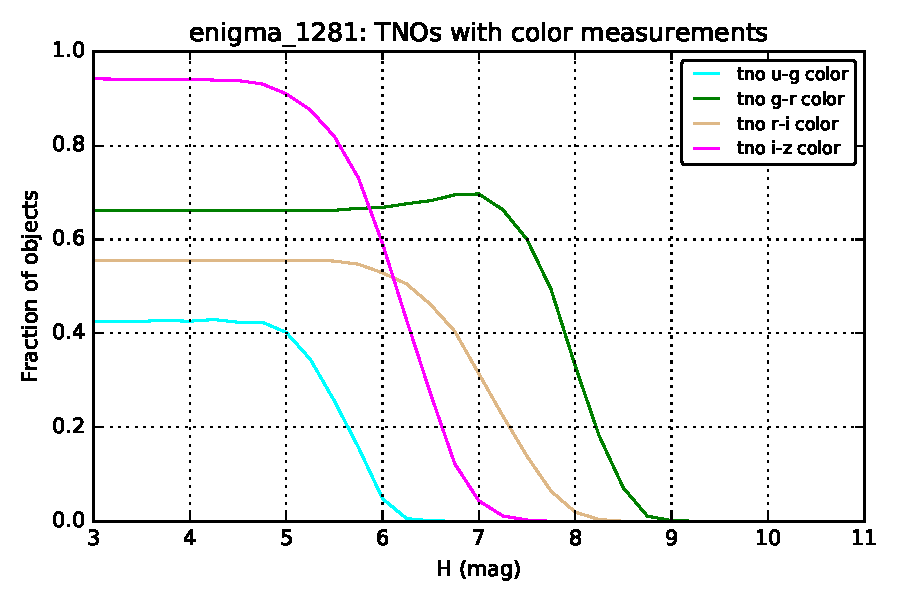
\includegraphics[width=3.3in]{figs/solarsystem/enigma_1281_ColorDetermination_i-z_u-g_r-i_g-r_color_tno_MOOB_ComboMetricVsH}
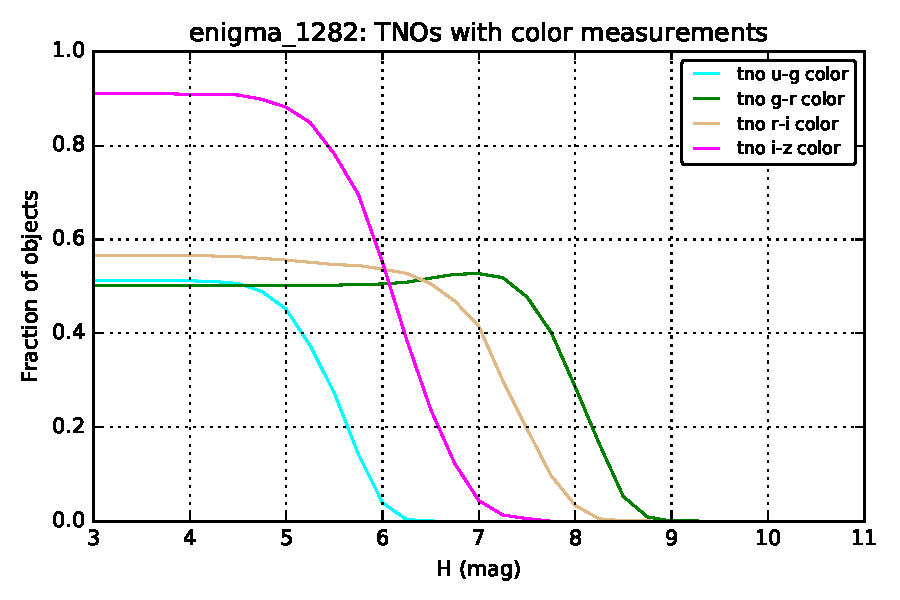
\includegraphics[width=3.3in]{figs/solarsystem/enigma_1282_ColorDetermination_i-z_u-g_r-i_g-r_color_tno_MOOB_ComboMetricVsH}
\caption{Fraction of the sample population with the potential for
  color measurements in various bands, as a function of $H$ magnitude
  for TNOs for simulated surveys \opsimdbref{db:baseCadence},
  \opsimdbref{db:NoVisitPairs}, \opsimdbref{db:NEOswithVisitTriplets}
  and \opsimdbref{db:NEOwithVisitQuads}. The fraction of TNOs which
  could receive high accuracy color measurements, particularly in
  $r-i$, bounces around significantly.
\label{colordetermination}}
\end{figure}

The timing of repeat visits, and whether or not filter changes occur
between these repeat visits, affects the fraction of objects which can
receive color measurements with closely spaced observations
significantly. This can be seen in the metric results shown in
Figure~\ref{colordetermination}. The difference is most pronounced in
the $r-i$ color measurements. The baseline survey,
\opsimdbref{db:baseCadence}, seems to perform rather well --- and
indeed, the best out of this set of runs.


% --------------------------------------------------------------------

\subsection{Discussion}
\label{sec:\secname:discussion}

This metric does not yet account for potential linking difficulties
related to identifying that these two observations are part of a
particular object, and it should be developed further to determine
appropriate parameters for objects other than TNOs, as other objects
may have different ranges of rotation rates. In particular, the
timescales needed when obtaining observations in multiple filters to
determine colors need to be explored.

There is some tension between desiring to get observations in the same
bandpass on a given night (to maximize detection thresholds instead
of being limited by the shallower bandpass) and obtaining color
measurements by having observations in multiple bandpasses. The risk
here is that without at least some nights with multi-band observations
on short timescales, we may not be able to determine accurate colors.

% --------------------------------------------------------------------

\navigationbar
